% $Header: /cvsroot/latex-beamer/latex-beamer/solutions/generic-talks/generic-ornate-15min-45min.en.tex,v 1.5 2007/01/28 20:48:23 tantau Exp $

\documentclass{beamer}

\usepackage{caption}
\captionsetup{labelformat=empty,labelsep=none,font=scriptsize}
\setlength{\abovecaptionskip}{0pt}

\usepackage{color}
%% These definitions are based on darkred at
%% http://www.december.com/html/spec/colorcmyk.html
\definecolor{darkred}{cmyk}{0, 1, 1, 0.45}
\newcommand{\jul}{\textcolor{darkred}}
\newcommand{\jan}{\textcolor{blue}}

% This file is a solution template for:

% - Giving a talk on some subject.
% - The talk is between 15min and 45min long.
% - Style is ornate.



% Copyright 2004 by Till Tantau <tantau@users.sourceforge.net>.
%
% In principle, this file can be redistributed and/or modified under
% the terms of the GNU Public License, version 2.
%
% However, this file is supposed to be a template to be modified
% for your own needs. For this reason, if you use this file as a
% template and not specifically distribute it as part of a another
% package/program, I grant the extra permission to freely copy and
% modify this file as you see fit and even to delete this copyright
% notice. 


\mode<presentation>
{
  \usetheme{Warsaw}
  % or ...

  \setbeamercovered{transparent}
  % or whatever (possibly just delete it)
}


\usepackage[english]{babel}
% or whatever

\usepackage[latin1]{inputenc}
% or whatever

\usepackage{times}
\usepackage[T1]{fontenc}
% Or whatever. Note that the encoding and the font should match. If T1
% does not look nice, try deleting the line with the fontenc.


%% \title[Short Paper Title] % (optional, use only with long paper titles)
%% {Presentation Title}
%% \title[]{Initial findings}
%\subtitle {Eastern CASTNET sites, May-Sep.~2001} % (optional)

%% \author[Author, Another] % (optional, use only with lots of authors)
%% {F.~Author\inst{1} \and S.~Another\inst{2}}
%% % - Use the \inst{?} command only if the authors have different
%% %   affiliation.
%% \author[Swall et al.]{Jenise Swall\inst{1}, Ana Rappold\inst{2}, and Lucas Neas\inst{2}
% - Use the \inst{?} command only if the authors have different
%   affiliation.

%% \institute[Universities of Somewhere and Elsewhere] % (optional, but mostly needed)
%% {
%%   \inst{1}%
%%   Department of Computer Science\\
%%   University of Somewhere
%%   \and
%%   \inst{2}%
%%   Department of Theoretical Philosophy\\
%%   University of Elsewhere}
%% % - Use the \inst command only if there are several affiliations.
%% % - Keep it simple, no one is interested in your street address.
 %% \institute[VCU]
 %% {
 %%   \inst{1}%
 %%   Dept.\ of Statistical Sciences and Operations Research\\
 %%   Virginia Commonwealth University
 %%   \and
 %%   \inst{2}%
 %%   National Health and Environmental Effects Research Laboratory\\
 %%   U.S.~Environmental Protection Agency
 %% }

%% \date[Short Occasion] % (optional)
%% {Date / Occasion}
\date{November 2021}

%% \subject{Talks}
% This is only inserted into the PDF information catalog. Can be left
% out. 



% If you have a file called "university-logo-filename.xxx", where xxx
% is a graphic format that can be processed by latex or pdflatex,
% resp., then you can add a logo as follows:

% \pgfdeclareimage[height=0.5cm]{university-logo}{university-logo-filename}
% \logo{\pgfuseimage{university-logo}}



% Delete this, if you do not want the table of contents to pop up at
% the beginning of each subsection:
\AtBeginSection[]
{
  \begin{frame}<beamer>{Outline}
    \tableofcontents[currentsection,currentsubsection]
  \end{frame}
}


% If you wish to uncover everything in a step-wise fashion, uncomment
% the following command: 

%\beamerdefaultoverlayspecification{<+->}

\useoutertheme{infolines}

\begin{document}

%% \begin{frame}
%%   \titlepage
%% \end{frame}

%% \begin{frame}{Outline}
%%  \tableofcontents
  % You might wish to add the option [pausesections]
%% \end{frame}


% Since this a solution template for a generic talk, very little can
% be said about how it should be structured. However, the talk length
% of between 15min and 45min and the theme suggest that you stick to
% the following rules:  

% - Exactly two or three sections (other than the summary).
% - At *most* three subsections per section.
% - Talk about 30s to 2min per frame. So there should be between about
%   15 and 30 frames, all told.


%% %%%%%%%%%%%%%%%%%%%%%%%%%%%%%%%%%%%%%%%%%%%%%%%%%%%%%%%%%%



%% %%%%%%%%%%%%%%%%%%%%%%%%%%%%%
%% Introductory material
%% \section[Background]{Background ideas and info}
\section[Preparation]{Preparing the data}



\begin{frame}{Percentages unclassified at the family level}

  \begin{center}
    \begin{figure}
      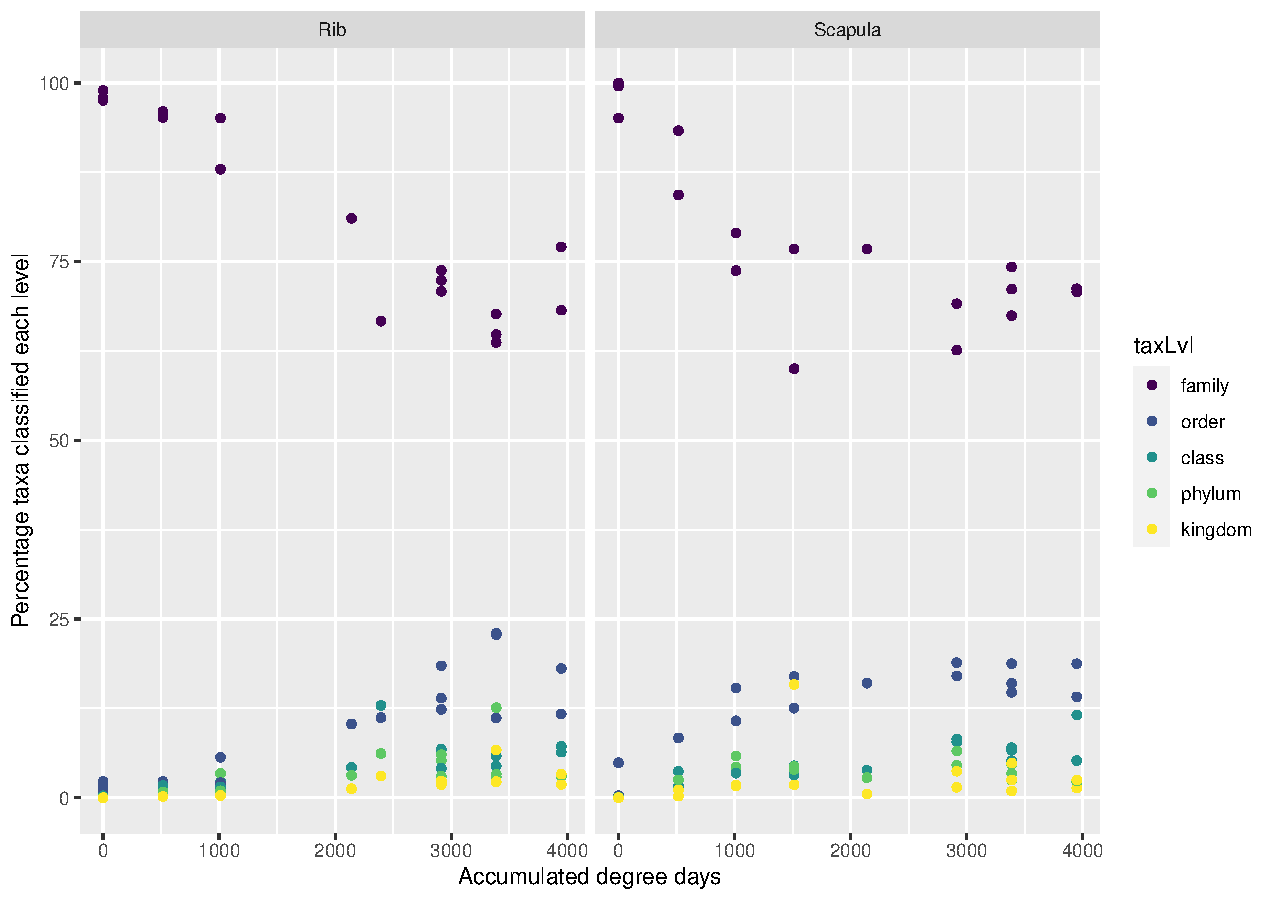
\includegraphics[width=3.25in]{swabs_family_perc_classif_by_add_type}
    \end{figure}
  \end{center}
  \vspace{-0.1in}
  {\footnotesize
  Fractions classified to family level:
  \begin{itemize}
    \item Ribs: 83.6\% (vs.\ 83.8\% for bones)
    \item Scapulae: 77.9\% (vs.\ 78.9\% for bones)
  \end{itemize}
  }
\end{frame}


\begin{frame}{Which taxa were included?}

  \begin{itemize}
  \item For each sample, we calculated the total counts of all classified,
family-level taxa.
  \item For each sample, we calculated the fraction of counts
associated with each family-level taxa. 
  \item To be included in the family-level analysis, we require that a taxon
  makes up more than 1\% of the total counts for at least 2 samples.
  \end{itemize}

  \vspace{0.1in}

  \noindent This is similar to the process we used when setting up for the
analyses in the Forger et al.~ paper, but I'm open to revisiting it.

  \vspace{0.1in}

  \noindent Number of taxa utilized in random forest models:
  \begin{itemize}
    \item Ribs: 49 taxa (vs.\ 41 used for earlier bone analysis)
    \item Scapulae: 53 taxa (vs.\ 55 used for earlier bone analysis)
  \end{itemize}


\end{frame}
%% %%%%%%%%%%%%%%%%%%%%%%%%%%%%%



%% %%%%%%%%%%%%%%%%%%%%%%%%%%%%%
\section[Rib swabs]{Working with swabs from ribs}


\begin{frame}{Implementing the random forest model for ribs (omitting baseline obs)}

  \noindent Full model omitting baseline observations (not using ADD 0):
  \begin{itemize}
    \item Utilized 49 family-level taxa.
    \item RMSE: $\approx$ 642.7  
    \item Explained variation: $\approx$ 73.1\%
  \end{itemize}
  % RMSE went down from about 670 and expl. variation up from about 72 after
  % dataset updated.
  \vspace{0.1in}

  \noindent We have 15 observations for the rib swabs when we exclude the
  baseline observations (as compared with 13 before the dataset was updated).
  % Compared with 13 observations before dataset updated.

\end{frame}



\begin{frame}{Implementing the random forest model for ribs (using baseline obs)}

  \noindent Full model using baseline observations (using ADD 0):
  \begin{itemize}
    \item Utilized 49 family-level taxa.
    \item RMSE: $\approx$ 600.6  
    \item Explained variation: $\approx$ 82.2\%
  \end{itemize}
  
  \vspace{0.1in}

  \noindent We have 18 observations for the rib swabs when we include the
  baseline observations.

\end{frame}
% %%%%%%%%%%%%%%%%%%%%%%%%%%%%%




% %%%%%%%%%%%%%%%%%%%%%%%%%%%%%
\section[Scapula swabs]{Working with swabs from scapulae}

\begin{frame}{Implementing the random forest model for scapulae (omitting baseline obs)}

  \noindent Full model omitting baseline observations (not using ADD 0):
  \begin{itemize}
    \item The model utilized 53 family-level taxa. % same as before update
    \item RMSE: $\approx$ 800.9
    \item Explained variation: $\approx$ 56.6\%
  \end{itemize}
  % RMSE is up from 771.2.  Expl. variation is down from 59.8.
  \vspace{0.1in}

  \noindent We have 14 observations for the scapula swabs when baseline
  observations are excluded.
  % Also had 14 observations before dataset was updated.

\end{frame}


\begin{frame}{Implementing the random forest model for scapulae (using baseline obs)}

  \noindent Full model omitting baseline observations (using ADD 0):
  \begin{itemize}
    \item The model utilized 53 family-level taxa. 
    \item RMSE: $\approx$ 681.4
    \item Explained variation: $\approx$ 76.6\%
  \end{itemize}
  \vspace{0.1in}

  \noindent We have 17 observations for the scapula swabs when we include the
  baseline observations.

\end{frame}
% %%%%%%%%%%%%%%%%%%%%%%%%%%%%%



% %%%%%%%%%%%%%%%%%%%%%%%%%%%%%
\section[Swabs from ribs and scapulae]{Comparing rib and scapula models (swabs)}


% %%%%%
\subsection[No baseline]{Omitting baseline observations}

\begin{frame}{Influential taxa for swabs (without baseline obs.)}

  \begin{center}
    \begin{figure}
      \includegraphics[width=4.25in]
        {use_families/rr_swabs_rib_scapula_family_no_baseline_4panels}
    \end{figure}
  \end{center}

\end{frame}


\begin{frame}{Pred.\ vs. actual ADD for swabs (without baseline obs.)}

  \begin{center}
    \begin{figure}
      \includegraphics[width=4.75in]
        {use_families/rr_swabs_rib_scapula_family_no_baseline_predicted_vs_actual_ADD}
    \end{figure}
  \end{center}

\end{frame}
% %%%%%


% %%%%%
\subsection[With baseline]{Using baseline observations}

\begin{frame}{Influential taxa for swabs (with baseline obs.)}

  \begin{center}
    \begin{figure}
      \includegraphics[width=4.25in]
        {use_families/rr_swabs_rib_scapula_family_w_baseline_4panels}
    \end{figure}
  \end{center}

\end{frame}


\begin{frame}{Pred.\ vs. actual ADD for swabs (with baseline obs.)}

  \begin{center}
    \begin{figure}
      \includegraphics[width=4.75in]
        {use_families/rr_swabs_rib_scapula_family_w_baseline_predicted_vs_actual_ADD}
    \end{figure}
  \end{center}

\end{frame}
% %%%%%

% %%%%%%%%%%%%%%%%%%%%%%%%%%%%%



% %%%%%%%%%%%%%%%%%%%%%%%%%%%%%
\section[Bones vs.\ swabs]{Comparing models using bones vs.\ swabs}

% %%%%%%%%%%
% %%%%%
\subsection[Ribs]{Using ribs}


% %%%%%
\subsubsection[No baseline]{Omitting baseline observations}

\begin{frame}{Ribs: Influential taxa (no baseline obs.)}

  \begin{center}
    \begin{figure}
      \includegraphics[width=4.25in]
        {../../rr_rib_bones_vs_swabs_no_baseline_4panels}
    \end{figure}
  \end{center}

\end{frame}


\begin{frame}{Ribs: Pred.\ vs. actual ADD (no baseline obs.)}

  \begin{center}
    \begin{figure}
      \includegraphics[width=4.75in]
        {../../rr_rib_bones_vs_swabs_no_baseline_predicted_vs_actual_ADD}
    \end{figure}
  \end{center}

\end{frame}
% %%%%%


% %%%%%
\subsubsection[With baseline]{Using baseline observations}

\begin{frame}{Ribs: Influential taxa (with baseline obs.)}

  \begin{center}
    \begin{figure}
      \includegraphics[width=4.25in]
        {../../rr_rib_bones_vs_swabs_w_baseline_4panels}
    \end{figure}
  \end{center}

\end{frame}


\begin{frame}{Ribs: Pred.\ vs. actual ADD (with baseline obs.)}

  \begin{center}
    \begin{figure}
      \includegraphics[width=4.75in]
        {../../rr_rib_bones_vs_swabs_w_baseline_predicted_vs_actual_ADD}
    \end{figure}
  \end{center}

\end{frame}
% %%%%%
% %%%%%%%%%%



% %%%%%%%%%%
% %%%%%%%%%%
% %%%%%
\subsection[Scapulae]{Using scapulae}

% %%%%%
\subsubsection[No baseline]{Omitting baseline observations}

\begin{frame}{Scapulae: Influential taxa (no baseline obs.)}

  \begin{center}
    \begin{figure}
      \includegraphics[width=4.25in]
        {../../rr_scapula_bones_vs_swabs_no_baseline_4panels}
    \end{figure}
  \end{center}

\end{frame}


\begin{frame}{Scapulae: Pred.\ vs. actual ADD (no baseline obs.)}

  \begin{center}
    \begin{figure}
      \includegraphics[width=4.75in]
        {../../rr_scapula_bones_vs_swabs_no_baseline_predicted_vs_actual_ADD}
    \end{figure}
  \end{center}

\end{frame}
% %%%%%


% %%%%%
\subsubsection[With baseline]{Using baseline observations}

\begin{frame}{Scapulae: Influential taxa (with baseline obs.)}

  \begin{center}
    \begin{figure}
      \includegraphics[width=4.25in]
        {../../rr_scapula_bones_vs_swabs_w_baseline_4panels}
    \end{figure}
  \end{center}

\end{frame}


\begin{frame}{Scapulae: Pred.\ vs. actual ADD (with baseline obs.)}

  \begin{center}
    \begin{figure}
      \includegraphics[width=4.75in]
        {../../rr_scapula_bones_vs_swabs_w_baseline_predicted_vs_actual_ADD}
    \end{figure}
  \end{center}

\end{frame}
% %%%%%



% %%%%%%%%%%
% %%%%%%%%%%%%%%%%%%%%%%%%%%%%%

\end{document}
